% ---------------------------------------------------------------------------
%  An Open Bitstream Pipeline for the ALINX AX7020
%  Tutorial, companion to https://maxclerkwell.tech/alinx/
%  Build: make   (XeLaTeX via latexmk; needs Inter and JetBrains Mono)
% ---------------------------------------------------------------------------
\documentclass[11pt,a4paper,oneside]{article}

% ---- Fonts: same faces as maxclerkwell.tech --------------------------------
\usepackage{fontspec}
\setmainfont{Inter}[
  UprightFont = *-Regular, BoldFont = *-SemiBold,
  ItalicFont = *-Italic, BoldItalicFont = *-SemiBoldItalic,
  Scale = 0.96]
\setsansfont{Inter}[UprightFont = *-Regular, BoldFont = *-SemiBold, Scale = 0.96]
\setmonofont{JetBrains Mono}[Scale = 0.86]
\newfontfamily\displayfont{Inter Display}[UprightFont = *-Medium, BoldFont = *-SemiBold]

% ---- Colours: the site palette on a white page -----------------------------
\usepackage{xcolor}
\definecolor{bochum}{HTML}{005BA1}     % headings, rules
\definecolor{bluemid}{HTML}{0072C8}
\definecolor{bright}{HTML}{1A9FFF}     % links
\definecolor{ink}{HTML}{0C1020}        % body text
\definecolor{muted}{HTML}{3F5870}      % secondary text
\definecolor{pale}{HTML}{C5DCF5}
\definecolor{codebg}{HTML}{F3F6FB}
\definecolor{codeframe}{HTML}{D9E4F2}
\definecolor{green}{HTML}{14803A}      % checkpoint accents
\definecolor{greenbg}{HTML}{EDF8F0}
\definecolor{amber}{HTML}{9A6700}
\definecolor{amberbg}{HTML}{FFF8E5}
\color{ink}

% ---- Page --------------------------------------------------------------------
\usepackage[a4paper, top=26mm, bottom=26mm, left=24mm, right=24mm]{geometry}
\usepackage{setspace}\setstretch{1.12}
\usepackage{microtype}
\usepackage{parskip}
\usepackage{booktabs, array, tabularx, longtable}
\usepackage{graphicx}
\usepackage{enumitem}
\setlist{itemsep=2pt, topsep=3pt, leftmargin=1.4em}
\newlist{filelist}{description}{1}
\setlist[filelist]{style=nextline, leftmargin=1.2em, labelindent=0pt, itemsep=5pt, topsep=4pt, font=\normalfont}
\usepackage{fontawesome5}
\usepackage{fancyhdr}
\usepackage{lastpage}
\usepackage{tikz}
\usetikzlibrary{arrows.meta, positioning, calc, shapes.misc}

% ---- Headings ----------------------------------------------------------------
\usepackage{titlesec}
\titleformat{\section}
  {\displayfont\color{bochum}\LARGE\bfseries}{\thesection}{0.7em}{}
  [{\color{bochum}\titlerule[0.8pt]}]
\titlespacing*{\section}{0pt}{22pt}{10pt}
\titleformat{\subsection}
  {\displayfont\color{bochum}\large\bfseries}{\thesubsection}{0.6em}{}
\titlespacing*{\subsection}{0pt}{14pt}{5pt}
\titleformat{\subsubsection}
  {\color{ink}\normalsize\bfseries}{\thesubsubsection}{0.6em}{}
\titlespacing*{\subsubsection}{0pt}{10pt}{3pt}

% ---- Header / footer ---------------------------------------------------------
\pagestyle{fancy}
\fancyhf{}
\renewcommand{\headrulewidth}{0pt}
\fancyhead[L]{\small\color{muted}An Open Bitstream Pipeline for the ALINX AX7020}
\fancyhead[R]{\small\color{muted}maxclerkwell.tech/alinx}
\fancyfoot[L]{\small\color{muted}Stephan Bökelmann (MaxClerkwell)}
\fancyfoot[R]{\small\color{muted}\thepage\,/\,\pageref{LastPage}}
\fancypagestyle{plain}{\fancyhf{}\renewcommand{\headrulewidth}{0pt}}

% ---- Code --------------------------------------------------------------------
\usepackage{listings}
\lstset{
  basicstyle=\ttfamily\small\color{ink},
  backgroundcolor=\color{codebg},
  frame=leftline, framerule=2pt, rulecolor=\color{bochum},
  framexleftmargin=6pt, xleftmargin=8pt, framesep=6pt,
  aboveskip=8pt, belowskip=8pt,
  breaklines=true, breakatwhitespace=true,
  columns=fullflexible, keepspaces=true,
  showstringspaces=false,
  keywordstyle=\color{ink}, commentstyle=\color{muted}, stringstyle=\color{ink},
  literate={ä}{{\"a}}1 {ö}{{\"o}}1 {ü}{{\"u}}1 {→}{{$\rightarrow$}}1 {─}{{-}}1 {│}{{|}}1 {▶}{{>}}1 {└}{{+}}1 {├}{{+}}1 {…}{{...}}1,
}
\lstdefinelanguage{none}{}
\lstnewenvironment{shell}{\lstset{language=bash}}{}
\lstnewenvironment{code}{\lstset{language=none}}{}
\usepackage{xurl}\urlstyle{tt}
\newcommand{\file}[1]{{\color{bluemid}\nolinkurl{#1}}}
\newcommand{\cmd}[1]{\texttt{#1}}

% ---- Boxes -------------------------------------------------------------------
\usepackage[most]{tcolorbox}
\newtcolorbox{checkpoint}[1][]{
  enhanced, breakable, colback=greenbg, colframe=green, boxrule=0pt,
  leftrule=3pt, arc=2pt, left=8pt, right=8pt, top=6pt, bottom=6pt,
  fonttitle=\bfseries, coltitle=green, colbacktitle=greenbg,
  title={\faCheckCircle\ Checkpoint#1}, attach title to upper={\ \ }, #1}
\newtcolorbox{note}{
  enhanced, breakable, colback=codebg, colframe=bochum, boxrule=0pt,
  leftrule=3pt, arc=2pt, left=8pt, right=8pt, top=6pt, bottom=6pt}
\newtcolorbox{mustknow}{
  enhanced, breakable, colback=amberbg, colframe=amber, boxrule=0pt,
  leftrule=3pt, arc=2pt, left=8pt, right=8pt, top=6pt, bottom=6pt,
  fonttitle=\bfseries, coltitle=amber,
  title={\faExclamationTriangle\ Rule}, attach title to upper={\ \ }}

% ---- Links -------------------------------------------------------------------
\usepackage[hidelinks]{hyperref}
\hypersetup{
  colorlinks=true, linkcolor=bochum, urlcolor=bright, citecolor=bochum,
  pdftitle={An Open Bitstream Pipeline for the ALINX AX7020},
  pdfauthor={Stephan Bökelmann (MaxClerkwell)},
  pdfsubject={Tutorial: mainline U-Boot over JTAG, Yocto Linux in QSPI, kexec updater, Yosys/nextpnr bitstreams and a REST API on a Zynq-7000 board, without vendor tools},
  pdfkeywords={Zynq, AX7020, ALINX, U-Boot, Yocto, kexec, Yosys, nextpnr, FPGA manager, FastAPI}}
\newcommand{\repo}{https://github.com/MaxClerkwell/ax7020-bringup}
\newcommand{\rfile}[1]{\href{\repo/blob/master/#1}{\color{bluemid}\nolinkurl{#1}}}
\newcommand{\lfile}[1]{\href{\repo/blob/master/yocto/meta-ax7020/#1}{\color{bluemid}\nolinkurl{#1}}}
\newcommand{\blog}[2]{\href{https://maxclerkwell.tech/posts/#1/}{#2}}
\newcommand{\series}{\href{https://maxclerkwell.tech/alinx/}{maxclerkwell.tech/alinx}}

\begin{document}

% =============================================================================
%  Title page
% =============================================================================
\begin{titlepage}
\thispagestyle{empty}
\begin{tikzpicture}[remember picture, overlay]
  \fill[bochum] (current page.north west) rectangle ([yshift=-9mm]current page.north east);
  \node[anchor=west, text=white, font=\small] at ([xshift=24mm, yshift=-4.5mm]current page.north west)
    {maxclerkwell.tech \quad·\quad Tutorial \quad·\quad September 2026};
\end{tikzpicture}

\vspace*{34mm}
{\color{muted}\small\textsc{Zynq-7000 · mainline U-Boot · Yocto · kexec · Yosys / nextpnr · REST}}

\vspace{5mm}
{\displayfont\color{bochum}\fontsize{30}{36}\selectfont\bfseries
An Open Bitstream Pipeline\\for the ALINX AX7020\par}

\vspace{6mm}
{\color{bochum}\rule{60mm}{1.2pt}}

\vspace{6mm}
{\large\color{ink}
From a blank board to a REST endpoint that accepts a bitstream and loads it
into the FPGA: JTAG bring-up with mainline U-Boot, a self-updating Yocto
Linux in QSPI flash, an open-toolchain bitstream, and a systemd-managed API.
No SD card, no serial cable, no vendor tool in the loop.\par}

\vspace{14mm}
{\displayfont\Large\bfseries Stephan Bökelmann}\\[1mm]
{\color{muted}MaxClerkwell \quad·\quad Bochum, Germany \quad·\quad nabla B}

\vspace{6mm}
\begin{tabular}{@{}l@{\hspace{7mm}}l@{}}
\faGlobe\ \href{https://maxclerkwell.tech}{maxclerkwell.tech} &
\faGithub\ \href{https://github.com/maxclerkwell}{maxclerkwell}\\[1mm]
\faTwitter\ \href{https://x.com/maxclerkwell}{@MaxClerkwell} &
\faLinkedin\ \href{https://www.linkedin.com/in/accelerator-stephan/}{accelerator-stephan}\\[1mm]
\faYoutube\ \href{https://www.youtube.com/@MaxClerkwell}{@MaxClerkwell} &
\faInstagram\ \href{https://www.instagram.com/_maxclerkwell/}{@\_maxclerkwell}\\[1mm]
\faDiscord\ \href{https://discord.gg/2BXuUY6hrX}{Full Stack Engineering} &
\faEnvelope\ \href{mailto:stephan@boekelmann.net}{stephan@boekelmann.net}
\end{tabular}

\vfill
\begin{minipage}{0.56\textwidth}
\small\color{muted}
Companion document to the five-part article series at \series.
All sources, recipes and scripts: \href{\repo}{github.com/MaxClerkwell/ax7020-bringup}.\\
The board was provided by \href{https://www.alinx.com/}{ALINX}; the vendor had no
influence on the content.
\end{minipage}
\hfill
\begin{minipage}{0.38\textwidth}
\raggedleft\small\color{muted}
Version 1.0\\
15 September 2026\\
Board: AX7020, XC7Z020-2CLG400
\end{minipage}
\end{titlepage}

% =============================================================================
\tableofcontents
\clearpage

% =============================================================================
\section{What this tutorial builds}

The ALINX AX7020 is a Zynq-7000 development board: two Cortex-A9 cores, a
7-series FPGA fabric on the same die, 1\,GiB of DDR3, 32\,MiB of QSPI flash and
Gigabit Ethernet on the processor side. The vendor path to a running system
goes through Vivado, the Xilinx FSBL, PetaLinux and an SD card. This tutorial
takes the other path and replaces every one of those with a component whose
source you can read.

\begin{center}
\resizebox{\textwidth}{!}{%
\begin{tikzpicture}[
  box/.style={draw=bochum, line width=0.8pt, rounded corners=2pt, fill=codebg,
              text width=35mm, align=center, minimum height=14mm, inner sep=2pt, font=\small},
  lab/.style={font=\scriptsize\color{muted}, align=center, text width=34mm},
  arr/.style={-{Stealth[length=2mm]}, line width=0.8pt, draw=bochum}]
  \node[box] (spl) at (0,0)     {mainline U-Boot\\SPL + proper\\{\scriptsize in QSPI}};
  \node[box] (mnt) at (5.0,0)   {maintenance Linux\\{\scriptsize Yocto FIT in QSPI}\\{\scriptsize systemd}};
  \node[box] (api) at (10.0,0)   {API image\\{\scriptsize in RAM, via kexec}\\{\scriptsize FastAPI on :8000}};
  \node[box] (pl)  at (15.0,0)  {FPGA fabric\\{\scriptsize /sys/class/}\\{\scriptsize fpga\_manager}};
  \draw[arr] (spl) -- node[lab, above=1pt, text width=14mm] {bootm} (mnt);
  \draw[arr] (mnt) -- node[lab, above=1pt, text width=14mm] {manifest} node[lab, below=1pt, text width=14mm] {kexec} (api);
  \draw[arr] (api) -- node[lab, above=1pt, text width=14mm] {POST} node[lab, below=1pt, text width=14mm] {/bitstream} (pl);
  \node[lab] at (0,-1.35)    {loaded once\\over JTAG};
  \node[lab] at (5.0,-1.35)  {flashed once\\over TFTP};
  \node[lab] at (10.0,-1.35)  {fetched on\\every boot};
  \node[lab] at (15.0,-1.35) {Yosys · nextpnr\\· prjxray};
\end{tikzpicture}}
\end{center}

When you are done, this is what a power cycle looks like, with nothing
attached but power and Ethernet:

\begin{code}
U-Boot: DHCP client bound to address 10.42.100.153
U-Boot: ## Loading kernel (any) from FIT Image at 02000000 ...
maintenance system -> ax7020-update.service -> image server -> kexec
API image: GET http://10.42.100.156:8000/state -> {"state":"unknown", ...}
POST blinky.bit -> {"state":"operating", "idcode":"0x03727093", ...}
\end{code}

\subsection{Scope}

This is the clean path: every command that is needed, in the order it is
needed, with a checkpoint after each step. The reasons behind the design
decisions, and the considerable number of ways each step can go wrong, are
in the article series at \series. Where a fact from that series is
\emph{required} to get through a step, it appears here as a rule; where it is
merely interesting, it does not.

\subsection{What you need}

\begin{itemize}
  \item An ALINX AX7020 with its 12\,V supply and an Ethernet cable.
  \item A JTAG adapter. An FTDI FT232H breakout is enough; no reset or
        buffer-enable line is needed on this board.
  \item A Linux workstation (Debian 13 was used) with a second Ethernet port
        or USB NIC for a private lab network, roughly 100\,GB of free disk for
        Yocto, and a few hours of build time.
  \item A machine on the company or lab network that can run one nginx
        container. A router or NAS is ideal.
  \item No SD card, no USB-UART cable, no Vivado, no PetaLinux.
\end{itemize}

\subsection{Board facts used throughout}

\begin{center}\small
\begin{tabular}{@{}ll@{}}
\toprule
SoC & XC7Z020-2CLG400, JTAG IDCODE \cmd{0x23727093} \\
DDR3 & 2\,$\times$ MT41J256M16, 32-bit bus, 533\,MHz, 1\,GiB \\
QSPI & Winbond W25Q256, 32\,MiB, single chip select, MIO 1..6 \\
Ethernet & PS GEM0, RGMII on MIO 16..27, RTL8211E-VL PHY at address 1 \\
Boot jumper & \textbf{J13}: left = SD, middle = QSPI, right = JTAG \\
PL clock & 50\,MHz oscillator on pin U18 \\
PL LEDs & M14, M15, K16, J16, active high, LVCMOS33 \\
\bottomrule
\end{tabular}
\end{center}

\subsection{Repository}

Every file referenced below is in \href{\repo}{github.com/MaxClerkwell/ax7020-bringup}.
Paths in this document are relative to its root.

\begin{code}
uboot/          DTS, defconfig, ps7_init for the mainline U-Boot tree
openocd/        adapter definition and the JTAG bring-up script
tools/          netconsole shell, TFTP server, publish and flash scripts
yocto/          meta-ax7020 layer and the build setup script
bitstream/      open toolchain flow, blinky and empty designs, bit2bin.py
api/            the FastAPI service
docs/           session walkthroughs (German), longer than this tutorial
\end{code}

% =============================================================================
\section{Host setup}

\subsection{Toolchain and tools}

\begin{shell}
sudo apt install gcc-arm-none-eabi openocd python3 make git
sudo apt install gawk wget diffstat unzip texinfo gcc build-essential \
    chrpath socat cpio python3-pip python3-pexpect xz-utils debianutils \
    iputils-ping python3-git python3-jinja2 python3-subunit zstd lz4 file \
    locales libacl1
\end{shell}

The second line is Yocto's host dependency list for Debian. Note \cmd{lz4}
rather than the older \cmd{liblz4-tool}; Yocto still looks for the binary
under its old name \cmd{lz4c}, and \rfile{yocto/hostbin/lz4c} is a symlink
that covers this without root.

\subsection{JTAG adapter}

\rfile{openocd/ft232h.cfg} describes a bare FT232H. On FTDI chips the MPSSE
pin assignment is fixed in silicon (ADBUS0 = TCK, 1 = TDI, 2 = TDO, 3 = TMS),
so only idle levels and directions are declared:

\begin{code}
adapter driver ftdi
ftdi vid_pid 0x0403 0x6014
ftdi layout_init 0x0008 0x000b
adapter speed 1000
transport select jtag
\end{code}

\begin{shell}
openocd -f openocd/ft232h.cfg -f target/zynq_7000.cfg
\end{shell}

\begin{checkpoint}
The chain shows two TAPs and both cores:
\begin{code}
JTAG tap: zynq_pl.bs tap/device found: 0x23727093 (Xilinx, part 0x3727)
JTAG tap: zynq.cpu   tap/device found: 0x4ba00477 (ARM Ltd)
zynq.cpu0: hardware has 6 breakpoints, 4 watchpoints
zynq.cpu1: hardware has 6 breakpoints, 4 watchpoints
\end{code}
\end{checkpoint}

\subsection{Lab network}

For bring-up the board hangs on a private network behind the workstation.
A NetworkManager \emph{shared} connection provides DHCP and keeps the board
off the house network:

\begin{shell}
nmcli connection add type ethernet ifname <iface> con-name zynq-lab \
    ipv4.method shared ipv4.addresses 192.168.77.1/24 ipv6.method disabled
nmcli connection up zynq-lab
\end{shell}

Find the board's address with \cmd{ip neigh show dev <iface>} after it has
taken a lease.

\subsection{Console and TFTP}

There is no serial cable in this setup. U-Boot's console is its
\emph{netconsole} over UDP port 6666, and \rfile{tools/ncsh.py} is the shell
for it. \rfile{tools/tftpd.py} is an unprivileged TFTP server, so no system
service is needed:

\begin{shell}
tools/tftpd.py tftp 6969 &                  # serves the tftp/ directory
tools/ncsh.py <board-ip>                    # interactive
tools/ncsh.py <board-ip> "bdinfo" "sf probe 0 30000000 0"   # one-shot
\end{shell}

On the board, \cmd{setenv tftpdstp 6969} points \cmd{tftpboot} at that port.

% =============================================================================
\section{Stage 1: Mainline U-Boot in QSPI flash}

Mainline U-Boot has no AX7020 support. Four files teach it the board; they
are mirrored in \file{uboot/} and go into a checkout of U-Boot
\cmd{v2026.10-rc2} or later.

\subsection{The four files}

\begin{filelist}
  \item[\rfile{uboot/zynq-ax7020.dts}] \file{arch/arm/dts/}. Board description, every value derived from the vendor's hardware handoff and schematic.
  \item[\rfile{uboot/alinx_ax7020_defconfig}] \file{configs/}. Derived from \cmd{xilinx\_zynq\_virt\_defconfig}: netconsole, legacy network stack, TFTP put, md5sum; SPL FIT loading and the relocated SPL stack switched off.
  \item[\rfile{uboot/ps7_init_gpl.c}, \file{.h}] \file{board/xilinx/zynq/zynq-ax7020/}. The PS initialisation Vivado generates (PLLs, MIO, DDR timing), extracted from the vendor's XSA archive, which is a plain zip. Five declarations gained \cmd{(void)} for GCC 15.
\end{filelist}

Two edits complete it: add \cmd{zynq-ax7020.dtb} to
\file{arch/arm/dts/Makefile}, and give the default environment in
\file{include/configs/zynq-common.h} \cmd{ncip} = \cmd{255.255.255.255} and
\cmd{stdin}/\cmd{stdout}/\cmd{stderr} = \cmd{serial,nc}, so the netconsole is
armed before the environment is ever writable.

\begin{mustknow}
Two device-tree facts are mandatory on this board. \cmd{bootph-all} must be
on the flash node \emph{and} the QSPI controller, or SPL finds no chip select.
And \cmd{spi-rx-bus-width} must be \cmd{<1>}: quad read returns data three
bytes off inside SPL, and U-Boot proper will not show the fault.
\end{mustknow}

\subsection{Build}

The boot command is compiled in rather than stored in the environment,
because \cmd{saveenv} does not work in JTAG boot mode and long \cmd{setenv}
lines break over the netconsole. It reads 24\,MiB from the FIT partition:

\begin{code}
CONFIG_BOOTCOMMAND="sf probe 0 30000000 0; sf read 0x2000000 0x340000 0x1800000; bootm 0x2000000"
\end{code}

\begin{shell}
cd u-boot
make alinx_ax7020_defconfig
scripts/config --disable TOOLS_MKEFICAPSULE      # host tool needs gnutls
make olddefconfig
make -j$(nproc) CROSS_COMPILE=arm-none-eabi-
cp spl/boot.bin u-boot.img ../tftp/
\end{shell}

\begin{checkpoint}
\file{spl/boot.bin} (about 107\,kB, SPL with the Xilinx boot header) and
\file{u-boot.img} (about 1.1\,MB, legacy uImage) exist.
\end{checkpoint}

\subsection{Flash layout}

\begin{center}\small
\begin{tabular}{@{}llll@{}}
\toprule
Offset & Content & Slot & mtd \\
\midrule
\cmd{0x000000} & \file{boot.bin} & 1\,MiB & 0 \\
\cmd{0x100000} & \file{u-boot.img} & 2\,MiB & 1 \\
\cmd{0x300000} & environment + redundant copy & 256\,KiB & 2 \\
\cmd{0x340000} & FIT: kernel + DTB + initramfs & 28.75\,MiB & 3 \\
\bottomrule
\end{tabular}
\end{center}

The same map is in the Linux device tree, so the running Linux sees the
partitions as \file{/dev/mtd0..3}.

\subsection{Bring-up over JTAG}

Board cold, J13 on JTAG, power on. \rfile{openocd/load-uboot.cfg} loads SPL
into on-chip memory, waits for \cmd{ps7\_init} to bring up DDR, writes and
reads a DDR test word, loads U-Boot proper to \cmd{0x4000000}, verifies it
and jumps:

\begin{shell}
openocd -f openocd/ft232h.cfg -f target/zynq_7000.cfg -f openocd/load-uboot.cfg
\end{shell}

\begin{mustknow}
Load U-Boot proper only while \emph{SPL} is halted, with caches off. Loading
into DDR while a previous U-Boot proper is halted corrupts the image in
32-byte chunks through its enabled D-cache. And after any QSPI-mode boot, a
JTAG-mode power cycle is mandatory before loading over JTAG again:
\cmd{ps7\_init} is not idempotent.
\end{mustknow}

\begin{checkpoint}
Over the netconsole, \cmd{bdinfo} reports 1\,GiB of DRAM and
\cmd{sf probe 0 30000000 0} detects \cmd{w25q256} with 32\,MiB.
\end{checkpoint}

\subsection{Flash}

Only from a U-Boot that was JTAG-loaded onto a freshly power-cycled board in
JTAG mode. Sizes are the file sizes in hex
(\cmd{printf "\%x\textbackslash n" \$(stat -c \%s tftp/boot.bin)}):

\begin{shell}
tools/ncsh.py <ip> "setenv tftpdstp 6969" "sf probe 0 30000000 0" \
  "tftpboot 0x10000000 boot.bin" "tftpboot 0x11000000 u-boot.img" \
  "md5sum 0x10000000 <size_boot_bin>" "md5sum 0x11000000 <size_u_boot_img>"
tools/ncsh.py <ip> "sf erase 0 0x300000" \
  "sf write 0x10000000 0 <size_boot_bin>" \
  "sf write 0x11000000 0x100000 <size_u_boot_img>"
tools/ncsh.py <ip> "sf read 0x12000000 0 <size_boot_bin>" \
  "md5sum 0x12000000 <size_boot_bin>" \
  "sf read 0x13000000 0x100000 <size_u_boot_img>" \
  "md5sum 0x13000000 <size_u_boot_img>"
\end{shell}

\begin{checkpoint}
Both read-back MD5s equal the host's \cmd{md5sum} of the files. Nothing
counts as flashed until they do.
\end{checkpoint}

\subsection{Standalone boot}

Power off, J13 to QSPI, JTAG unplugged, power on.

\begin{checkpoint}
U-Boot appears on the netconsole by itself, with \cmd{modeboot = qspiboot}.
The JTAG adapter goes into the drawer; everything from here on happens over
Ethernet.
\end{checkpoint}

% =============================================================================
\section{Stage 3: A Yocto Linux in flash}

\emph{Stages are numbered as in the article series, where the image server of
Stage 2 ended up being built after the Linux of Stage 3.}

Everything Linux needs ships as one artefact: a FIT image holding kernel,
device tree and an initramfs, written into the FIT partition. The root
filesystem lives in RAM. This image is the \emph{maintenance system}: small,
rarely changed, and the thing that fetches everything else.

\subsection{Layers}

\cmd{scarthgap} (Yocto 5.0 LTS) throughout, as the newest branch meta-xilinx
supports:

\begin{shell}
cd yocto
for r in "https://git.yoctoproject.org/poky poky" \
         "https://github.com/Xilinx/meta-xilinx meta-xilinx" \
         "https://git.yoctoproject.org/meta-arm meta-arm" \
         "https://github.com/openembedded/meta-openembedded meta-openembedded"; do
    set -- $r; git clone --depth 1 -b scarthgap "$1" "$2"
done
\end{shell}

\rfile{yocto/meta-ax7020} is the board layer. Its parts, paths relative to it:

\begin{filelist}
  \item[\lfile{conf/machine/ax7020.conf}] requires meta-xilinx's \cmd{zynq-generic}, sets \cmd{KERNEL\_IMAGETYPE} to \cmd{fitImage}, declares no bootloader provider, and names \cmd{ax7020-initramfs} as the initramfs that goes into the FIT.
  \item[\lfile{recipes-kernel/linux/files/zynq-ax7020.dts}] the Linux device tree, including the flash partition map.
  \item[\lfile{recipes-kernel/linux/files/ax7020.cfg}] kernel fragment: Zynq FPGA manager, FPGA regions and overlays, netconsole, MTD and QSPI, kexec; graphics, sound, wireless and IPv6 off.
  \item[\lfile{recipes-core/images/ax7020-initramfs.bb}] the maintenance image: core-image-minimal as \cmd{cpio.gz} plus dropbear, curl, kexec-tools, the updater and the operator's SSH key.
  \item[\lfile{recipes-support/ax7020-ssh-key}] installs \file{authorized_keys} to \cmd{\$\{ROOT\_HOME\}}. Put your public key in \rfile{yocto/meta-ax7020/recipes-support/ax7020-ssh-key/files/authorized_keys} before building.
  \item[\rfile{yocto/setup-build.sh}] regenerates \file{build/conf} from version control: machine \cmd{ax7020}, \cmd{INIT\_MANAGER = "systemd"}, no bootloader from Yocto.
\end{filelist}

\subsection{Build}

\begin{shell}
source yocto/setup-build.sh
setsid nohup bitbake virtual/kernel > build.log 2>&1 &     # detached: a killed
tail -f build.log                                          # client kills the build
\end{shell}

The first build takes several hours. The FIT lands in
\file{yocto/build/tmp/deploy/images/ax7020/} as
\file{fitImage-ax7020-initramfs-ax7020-ax7020}; copy it to \file{tftp/fitImage}.

\begin{checkpoint}
\cmd{dumpimage -l tftp/fitImage} lists one configuration with a kernel, the
DTB \cmd{zynq-ax7020.dtb} and a ramdisk, each with a SHA256 hash. The FIT is
under 24\,MiB.
\end{checkpoint}

\subsection{Boot from RAM first}

From a JTAG-loaded U-Boot, before anything is written:

\begin{shell}
tools/ncsh.py <ip> "setenv tftpdstp 6969" "tftpboot 0x2000000 fitImage" "bootm 0x2000000"
\end{shell}

\begin{checkpoint}
Linux boots, takes a DHCP lease under hostname \cmd{ax7020}, and
\textbf{port 22 answers} with key-only login. Ping is not the test; a U-Boot
with a working network stack also answers ping.
\end{checkpoint}

\subsection{Flash the FIT}

\begin{shell}
tools/ncsh.py <ip> "setenv tftpdstp 6969" "tftpboot 0x2000000 fitImage" \
  "sf probe 0 30000000 0" "sf erase 0x340000 0x1CC0000" \
  "sf write 0x2000000 0x340000 <size_fit>" \
  "sf read 0x3000000 0x340000 <size_fit>" "md5sum 0x3000000 <size_fit>" \
  "md 0x3000000 4" "md 0x3800000 4"
\end{shell}

\begin{checkpoint}
The read-back MD5 matches, \emph{and} the words at two different offsets of
the read-back differ from each other. A flash whose address lines are shifted
can return a self-consistent, wrong image that passes a single checksum.
\end{checkpoint}

Power off, J13 on QSPI, power on.

\begin{checkpoint}
Linux boots from flash on its own and is reachable over SSH. At this point
the board can be moved from the lab network to the company network; it will
announce itself as \cmd{ax7020} to DHCP.
\end{checkpoint}

% =============================================================================
\section{Stage 2: The image server and the updater}

The maintenance system never changes what is in flash. On every boot it asks
one URL for a manifest, downloads kernel, device tree and initramfs, verifies
them and \cmd{kexec}s into the result. A broken image costs a power cycle,
not a reflash, because after the power cycle the maintenance system is back.

\subsection{Server}

One nginx container on a machine the board can reach, read-only, bound to
the LAN address only, serving a directory:

\begin{shell}
docker run -d --name ax7020-image-server --restart unless-stopped \
  -p 10.42.0.1:8080:80 \
  -v /srv/ax7020-images:/usr/share/nginx/html:ro \
  -v /etc/ax7020-image-server/default.conf:/etc/nginx/conf.d/default.conf:ro \
  --read-only --tmpfs /var/cache/nginx --tmpfs /var/run --tmpfs /tmp nginx:alpine
\end{shell}

\file{default.conf} contains \cmd{autoindex on;} and \cmd{disable\_symlinks off;}.
Every build gets a timestamped directory; \file{ax7020-latest} is a symlink to
the newest one. The board knows exactly one URL:

\begin{code}
http://10.42.0.1:8080/ax7020-latest/manifest
\end{code}

\subsection{Publishing}

\rfile{tools/publish-image.sh} copies zImage, DTB and \cmd{cpio.gz} from the
Yocto deploy directory over scp, writes the manifest with SHA256 sums, and
repoints the symlink:

\begin{shell}
tools/publish-image.sh AI-heimdall:/srv/ax7020-images                  # API image
tools/publish-image.sh -i ax7020-initramfs AI-heimdall:/srv/ax7020-images   # maintenance image
\end{shell}

\begin{code}
kernel zImage             542ef58f...
dtb    zynq-ax7020.dtb    1e3fa9c7...
initrd initramfs.cpio.gz  4e73ba34...
\end{code}

\begin{mustknow}
The manifest names three files, not a FIT. \cmd{kexec-tools} on 32-bit ARM
has no FIT loader and its zImage probe accepts any file; handed a FIT, it
jumps into the device tree and the board dies silently. The updater checks
the zImage magic at offset \cmd{0x24} and the DTB magic itself, because
nothing downstream will.
\end{mustknow}

\subsection{The updater}

The updater lives in \rfile{yocto/meta-ax7020/recipes-support/ax7020-updater/files/}:
\file{ax7020-update} is the shell script, \file{ax7020-update.conf} sets
\cmd{IMAGE\_URL} (empty means \emph{stay in the maintenance system}), and
\file{ax7020-update.service} runs it once per boot:

\begin{code}
[Unit]
After=network-online.target time-sync.target
Wants=network-online.target

[Service]
Type=oneshot
ExecStartPre=/bin/sleep 15
ExecStart=/usr/bin/ax7020-update
StandardOutput=journal+console
\end{code}

The script fetches the manifest, then each file, compares every SHA256, checks
both magics, and runs \cmd{kexec -l zImage --dtb --initrd --command-line} followed
by \cmd{kexec -e}. \cmd{DRY\_RUN=1} stops before the jump. If anything fails the
unit fails and the board stays reachable over SSH.

\begin{checkpoint}
Publish the maintenance image itself, set \cmd{IMAGE\_URL}, reboot: about
twenty seconds later the same system is back with an uptime of seconds, and
\cmd{journalctl -u ax7020-update} shows three checksums verified.
\end{checkpoint}

% =============================================================================
\section{Stage 4: A bitstream without Vivado}

\subsection{Toolchain}

The Zynq-7020 is a 7-series device and is covered by the openXC7 flow.
Everything except Yosys is built from source under \file{build/}:

\begin{center}\small
\begin{tabular}{@{}lll@{}}
\toprule
Tool & Source & Role \\
\midrule
Yosys 0.66 & Debian package & synthesis, \cmd{synth\_xilinx} \\
nextpnr-xilinx & openXC7 fork & placement and routing, reads XDC \\
prjxray & f4pga & \cmd{fasm2frames}, \cmd{xc7frames2bit} \\
prjxray-db & zynq7 & bitstream database, chipdb for \cmd{xc7z020} \\
\bottomrule
\end{tabular}
\end{center}

The chip database for the XC7Z020 is generated once from prjxray-db; it is
a few hundred megabytes and everything below depends on it.

\subsection{Design}

\rfile{bitstream/blinky/blinky.v}: a 27-bit counter on the 50\,MHz PL
oscillator, four LEDs on the top bits, and one line that is not optional:

\begin{code}
module blinky (input wire sys_clk, output wire [3:0] led);
    reg [26:0] cnt = 27'd0;
    always @(posedge sys_clk) cnt <= cnt + 27'd1;
    assign led = cnt[26:23];
    (* keep *) PS7 ps7_i();
endmodule
\end{code}

\begin{mustknow}
A Zynq design \textbf{must instantiate the PS7 block}, even if it uses
nothing of it. nextpnr then ties every unused PS7 input to ground. Without
it, the fabric drives the direct nFIQ/nIRQ lines into both Cortex-A9 cores
(\cmd{IRQF2P[19:16]}, which bypass the interrupt controller) the moment the
kernel enables the PL-to-PS level shifters. Both cores spin in FIQ handling
forever and nothing is ever printed.
\end{mustknow}

Pins come from \rfile{bitstream/blinky/blinky.xdc}, a plain XDC file that
nextpnr reads directly.

\subsection{Flow}

\rfile{bitstream/blinky/Makefile} chains four tools and one conversion:

\begin{code}
blinky.v  --yosys synth_xilinx-->  blinky.json
          --nextpnr-xilinx---->  blinky.fasm
          --fasm2frames------->  blinky.frames
          --xc7frames2bit----->  blinky.bit
          --bit2bin.py-------->  blinky.bin
\end{code}

\begin{shell}
cd bitstream/blinky && make blinky.bin
\end{shell}

The last step, \rfile{bitstream/bit2bin.py}, exists because the kernel's
\cmd{zynq-fpga} driver expects the layout \cmd{bootgen} produces: the ASCII
header of the \cmd{.bit} removed, every 32-bit word byte-swapped.

\begin{checkpoint}
\cmd{xxd -l 16 blinky.bin} shows \cmd{ffff ffff ffff ffff 6655 99aa}, the sync
word in swapped order.
\end{checkpoint}

\subsection{Load over SSH}

The FPGA manager takes a file \emph{name} relative to \file{/lib/firmware}:

\begin{shell}
ssh root@<ip> 'mkdir -p /lib/firmware; cat > /lib/firmware/blinky.bin' < blinky.bin
ssh root@<ip> 'echo blinky.bin > /sys/class/fpga_manager/fpga0/firmware;
               cat /sys/class/fpga_manager/fpga0/state'
\end{shell}

\rfile{tools/stage4-first-load/load-bitstream.sh} does the same with the
kernel log redirected to the workstation via netconsole, which is worth
having the first time.

\begin{checkpoint}
\cmd{state} reads \cmd{operating}, the four LEDs blink, and the board still
answers on port 22.
\end{checkpoint}

% =============================================================================
\section{Stage 5: The bitstream API as an image}

\subsection{The service}

\rfile{api/app.py} is a FastAPI application with three endpoints:

\begin{center}\small
\begin{tabularx}{\textwidth}{@{}llX@{}}
\toprule
\cmd{GET} & \file{/state} & FPGA manager state and what was loaded last \\
\cmd{POST} & \file{/bitstream} & multipart \cmd{file=}, \cmd{.bit} or \cmd{.bin}, optional \cmd{?sha256=}; verifies the checksum, finds the sync word, checks the IDCODE packet against the XC7Z020, converts a \cmd{.bit}, loads, answers when the fabric is up \\
\cmd{DELETE} & \file{/bitstream} & loads \file{empty.bin}, a PS7-only design, because the FPGA manager has no unload \\
\bottomrule
\end{tabularx}
\end{center}

The IDCODE check looks for the type-1 packet \cmd{0x30018001} in the header
and compares the following word, masked to 28 bits, with \cmd{0x23727093};
the top four bits are the silicon revision. Errors come back as
\cmd{\{"error": "..."\}} with 400 or 500. The interactive documentation is
served at \file{/docs}.

\subsection{Recipes}

All in \rfile{yocto/meta-ax7020}, paths relative to it:

\begin{filelist}
  \item[\lfile{classes/pypi-wheel.bbclass}] installs a pure-Python wheel by unzipping it into site-packages. scarthgap has no class for the \cmd{pdm-backend} that FastAPI's build metadata asks for, and a wheel is already the installed tree.
  \item[\file{recipes-devtools/python/}] fastapi 0.111.1, starlette 0.37.2, uvicorn 0.30.6, click 8.1.7, python-multipart 0.0.9 as wheels; pydantic, anyio and h11 from meta-python.
  \item[\lfile{recipes-devtools/uv/uv_0.12.13.bb}] astral's static armv7-musl binary, hash pinned, for \cmd{uv run --with ...} experiments on the board. Not in the service's start path.
  \item[\lfile{recipes-support/ax7020-api/ax7020-api.bb}] \file{app.py} to \file{/opt/ax7020-api}, \file{empty.bin} to \file{/lib/firmware}, and the unit below, enabled.
  \item[\lfile{recipes-core/images/ax7020-api-image.bb}] core-image-minimal plus the above, Python, dropbear and the operator key. \cmd{INITRAMFS\_MAXSIZE} raised to 512\,MB. \textbf{Without} the updater.
\end{filelist}

\rfile{yocto/meta-ax7020/recipes-support/ax7020-api/files/ax7020-api.service}:

\begin{code}
[Service]
Type=simple
WorkingDirectory=/opt/ax7020-api
ExecStart=/usr/bin/python3 -m uvicorn app:app --host 0.0.0.0 --port 8000
Restart=on-failure
RestartSec=3
\end{code}

\begin{mustknow}
The API image must not contain the updater. With \cmd{IMAGE\_URL} set it
would fetch itself and \cmd{kexec} into itself on every boot, forever.
\end{mustknow}

\subsection{Build, publish, and update the maintenance system}

\begin{shell}
source yocto/setup-build.sh
bitbake ax7020-api-image virtual/kernel        # API image + new maintenance FIT
tools/publish-image.sh AI-heimdall:/srv/ax7020-images
\end{shell}

The maintenance FIT with the systemd-based updater has to go into flash once
more. From the running Linux, over SSH, no jumper: \rfile{tools/flash-fit.sh}
uploads, writes through \file{/dev/mtdblock3}, reads back and compares three
MD5s. If U-Boot was rebuilt as well, the same script writes \file{u-boot.img}
to \file{/dev/mtdblock1}:

\begin{shell}
tools/flash-fit.sh <ip> tftp/fitImage          # mtd3, the FIT
tools/flash-fit.sh <ip> tftp/u-boot.img 1      # mtd1, U-Boot proper
\end{shell}

\begin{checkpoint}
All three MD5 lines printed by the script match: local file, upload, and
flash read-back.
\end{checkpoint}

\subsection{The cold boot}

Power off. \textbf{Unplug the JTAG adapter.} Power on.

\begin{mustknow}
An FT232H left on the JTAG port holds TMS at 3.3\,V and, through the
protection diodes, keeps the board's 3.3\,V rail and the flash chip alive
across a power cycle. A flash chip that a Linux session left in 4-byte
address mode then never resets, and the boot ROM, which reads with 3-byte
addresses, parks at \cmd{0xffffff28}. "Power-cycled" is only true with the
adapter unplugged.
\end{mustknow}

\begin{checkpoint}
Within about a minute, with nobody logged in, port 8000 answers on the
address the DHCP server holds for \cmd{ax7020}, and a bitstream goes in:
\begin{shell}
IP=$(curl -s http://10.42.0.1:8000/get_all_network_clients \
     | jq -r '.clients[] | select(.hostname=="ax7020" and .active_lease) | .ip')
curl http://$IP:8000/state
curl -F file=@bitstream/blinky/blinky.bit http://$IP:8000/bitstream
\end{shell}
\begin{code}
{"state":"operating", "sha256":"f69a32d2...", "bytes":4045524,
 "idcode":"0x03727093", "filename":"blinky.bit"}
\end{code}
\end{checkpoint}

% =============================================================================
\section{Operating the board}

\subsection{Finding it}

U-Boot, the maintenance kernel and the API kernel each take their own DHCP
lease, so the address changes across a boot. Query the DHCP server by
hostname rather than remembering an address. The inventory API used above is
\href{https://github.com/MaxClerkwell/dhcp-inventory-api}{dhcp-inventory-api};
any DHCP server's lease file works the same way.

\subsection{SSH}

The root filesystem is in RAM, so dropbear generates a new host key on every
boot. Before each session:

\begin{shell}
ssh-keygen -R <ip>
\end{shell}

\cmd{Connection refused} right after a boot means only that dropbear is not
up yet; key generation takes about 30\,s on this CPU.

\subsection{Rolling back an image}

On the image server, point \file{ax7020-latest} at an older directory and
power-cycle the board. Nothing in flash changes.

\subsection{Rewriting flash}

\rfile{tools/flash-fit.sh} for the FIT (mtd3) and U-Boot proper (mtd1), from
the running Linux. \file{boot.bin} (mtd0) is written only through the JTAG
procedure of Stage 1, and the environment (mtd2) belongs to U-Boot.

\subsection{Backing up flash}

From U-Boot, over TFTP:

\begin{shell}
tools/ncsh.py <ip> "sf probe 0 30000000 0" "sf read 0x10000000 0 0x2000000" \
  "md5sum 0x10000000 0x2000000" "tftpput 0x10000000 0x2000000 ax7020-qspi.bin"
\end{shell}

% =============================================================================
\section{Where to go from here}

The pipeline is complete as a lab system. Three additions turn it into
something that can face a wider network, in this order:

\begin{enumerate}
  \item \textbf{Authentication} on the API. A bitstream with an AXI master
        has full access to system memory; loading unreviewed bitstreams is
        remote code execution with extra steps.
  \item \textbf{A bitstream in the manifest.} A fourth line,
        \cmd{bitstream <file> <sha256>}, loaded by the service at start, so
        the fabric is never empty after boot.
  \item \textbf{A build stamp} in \file{/etc/ax7020-release}, reported by
        \file{/state}, so the running image can be told from the one in flash
        and the one on the server.
\end{enumerate}

The reasoning behind every decision in this document, and the detours that
produced the rules in the amber boxes, are in the five articles at \series:

\begin{itemize}
  \item \blog{zynq-bitstream-deployment-concept-august-2026}{Deploying Hardware Like Software: A Bitstream Pipeline for the Zynq}
  \item \blog{alinx-bring-up-jtag-detected-without-power-august-2026}{ALINX AX7020 Bring-up: Mainline U-Boot Over JTAG, No FSBL, No Serial Cable}
  \item \blog{alinx-ax7020-yocto-linux-qspi-august-2026}{Stages 2 \& 3: A Yocto Linux in QSPI Flash That Fetches Its Own Updates}
  \item \blog{alinx-ax7020-open-bitstream-rest-api-september-2026}{Stages 4 \& 5: An Open Bitstream Over REST, and the One Missing Line That Hangs Both Cores}
  \item \blog{alinx-ax7020-cold-boot-to-bitstream-api-september-2026}{Stage 5 Complete: Cold Power-On to a Bitstream API, Nobody Logged In}
\end{itemize}

% =============================================================================
\clearpage
\section*{About the author}
\addcontentsline{toc}{section}{About the author}

\begin{minipage}[t]{0.26\textwidth}
\vspace{0pt}
\begin{tikzpicture}
  \clip (0,0) circle (18mm);
  \node at (0,0) {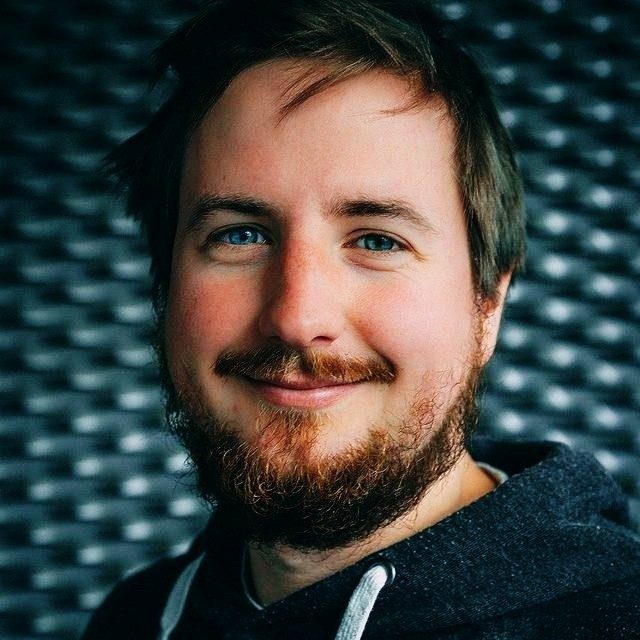
\includegraphics[width=36mm]{avatar.jpg}};
\end{tikzpicture}
\end{minipage}
\hfill
\begin{minipage}[t]{0.70\textwidth}
\vspace{0pt}
{\displayfont\Large\bfseries\color{bochum} Stephan Bökelmann}\\
{\color{muted}MaxClerkwell · Engineer, physicist, freelance consultant · Bochum, Germany}

\vspace{3mm}
Stephan works across the full vertical stack of engineering: silicon-level
measurement systems, embedded firmware, PCB design and bring-up, FPGA
development, and the monitoring and data infrastructure above them. The
common thread is decentralised data acquisition: getting reliable
measurements out of physical systems, whether that system is a particle
detector, a production line or a development board that has stopped
talking.

He is a trained mechanic and electrician, a state-certified mechanical
engineer, holds a B.Eng.\ in electrical engineering and an M.Eng.\ in
computer engineering, and is completing a PhD
in experimental hadron physics at Ruhr-Universität Bochum, working on HV-MAPS
sensors for the PANDA luminosity detector at FAIR. He is managing director of
the engineering office \href{https://nabla-b.engineering/}{nabla B}, COO of
AUTO INTERN and system architect of its skAInet Edge-Compute platform, and
lectures on programming and databases at THGA Bochum. He is the principal
organiser of emBO++, a co-organiser of KiCon Europe, and holds several
patents in measurement technology. Professionally active since 2007.
\end{minipage}

\vspace{8mm}
\begin{tcolorbox}[enhanced, colback=codebg, colframe=bochum, boxrule=0pt,
  leftrule=3pt, arc=2pt, left=10pt, right=10pt, top=8pt, bottom=8pt]
{\displayfont\large\bfseries\color{bochum} Available for projects}

\vspace{2mm}
Work like this tutorial is what I do professionally, through my company
nabla B in Bochum: board bring-up without vendor lock-in, embedded Linux with
Yocto and mainline U-Boot, FPGA development with open or vendor toolchains,
PCB design in KiCad from schematic to EMC, and data-acquisition systems from
the sensor to the server. On-site in the DACH region, remote worldwide, in
English or German, from feasibility study to serial product.

\vspace{3mm}
\begin{tabular}{@{}ll@{}}
\faEnvelope\ Commissioned work & \href{mailto:office@nabla-b.engineering}{office@nabla-b.engineering} \\
\faEnvelope\ Direct & \href{mailto:stephan@boekelmann.net}{stephan@boekelmann.net} \\
\faEnvelope\ Board vendors and collaborations & \href{mailto:collaboration@maxclerkwell.tech}{collaboration@maxclerkwell.tech} \\
\faBriefcase\ Services and references & \href{https://maxclerkwell.tech/hire/}{maxclerkwell.tech/hire} \\
\faLinkedin\ LinkedIn & \href{https://www.linkedin.com/in/accelerator-stephan/}{linkedin.com/in/accelerator-stephan} \\
\end{tabular}
\end{tcolorbox}

\vspace{6mm}
{\small\color{muted}
Blog and article series: \href{https://maxclerkwell.tech}{maxclerkwell.tech} · \series\\
Sources for this tutorial: \href{\repo}{github.com/MaxClerkwell/ax7020-bringup}\\
Discord, Full Stack Engineering: \href{https://discord.gg/2BXuUY6hrX}{discord.gg/2BXuUY6hrX}\\[2mm]
\faCreativeCommons\ \faCreativeCommonsBy\ This document is licensed under
\href{https://creativecommons.org/licenses/by/4.0/}{Creative Commons Attribution 4.0 (CC BY 4.0)}:
use, share and adapt it freely, with attribution to Stephan Bökelmann
(MaxClerkwell) and a link to \series. The AX7020 was provided by ALINX as a
sponsorship; the vendor had no influence on its content.}

\end{document}
